\documentclass[a4paper,english,fleqn]{exam}

\usepackage{babel} % voor nederlandse afbreekregels e.d.
\usepackage{hyperref} % voor links, hier niet gebruikt
\usepackage{graphicx} % voor importeren van figures, hier niet gebruikt
\usepackage{tabularx} % voor tabellen met controle over kolombreedte, hier niet gebruikt
\usepackage{booktabs} % voor nettere tabellen dan de standaard
\usepackage{enumerate} % voor controle over nummering van items
\usepackage{amssymb,amsmath,amsthm,amsfonts} % van de AMS, voor nettere math
\usepackage{qtree} % voor het maken van mooie bomen, hier niet gebruikt
\usepackage{mathabx} %voor het \notdivides commando, niet gebruikt
\usepackage{adjustbox}
\usepackage{listings}
\usepackage{color}
\usepackage{wrapfig}


\usepackage{pifont}
\usepackage{algorithm} % pseudocode
\usepackage[noend]{algpseudocode} %pseudocode 
\usepackage{sectsty}

\renewcommand\thesubsection{\thesection \alph{subsection}}
\newcommand{\s}{\text{*}}

%\DeclareGraphicsExtensions{.pdf,.png,.jpg}


\renewcommand{\baselinestretch}{0.9} 

\sectionfont{\fontsize{14}{17}\selectfont}

\renewcommand{\qedsymbol}{\hfill \emph{QED}}

% document variables:
\newcommand{\cMysename}{TI2806 Contextproject }
\newcommand{\doctitle}{Emergent Architecture \\ Group HI4 }
\newcommand{\deadline}{May 22 2015}
\newcommand{\examdate}{\deadline}
\newcommand{\authors}{Group HI4}
% ---

\newcommand{\cmark}{\ding{51}}%
\newcommand{\xmark}{\ding{55}}%

\newcommand{\itab}[1]{\hspace{0em}\rlap{#1}}
\newcommand{\tab}[1]{\hspace{.2\textwidth}\rlap{#1}}

% http://tex.stackexchange.com/questions/110328/formatting-a-logical-pd-derivation:
\newcommand{\fgh}[1]{\fvline%
  \makebox[0pt][l]{{%
      \raisebox{-1.4ex}[0pt][0pt]{\rule{#1}{\arrayrulewidth}}}}%
  \hspace*{\fitchindent}}
  
  \lstset{language=Java,
%alles tussen "//(*" en "*)" wordt als TeX code verIrkt
	escapeinside={//(*}{*)}} 
 


\newcommand*\xor{\mathbin{\oplus}}
% Fill these in:

% if you use algorithms, this is a nice one:
% http://www.lirmm.fr/~fiorio/AlgorithmSty/
%\usepackage[algo2e]{algorithm2e}


% http://detexify.kirelabs.org/classify.html

% Use Sans-Serif font:
\usepackage{helvet}
\renewcommand{\familydefault}{\sfdefault}

\addpoints % Sum totals per question
\totalformat{Vraag \thequestion: \totalpoints\ \points}
\headrule
\header{\cMysename}{\doctitle}{\deadline}
\footrule
\footer{\authors}{\iflastpage{End of report}{}}{\thepage\ of \numpages}

\coverextraheadheight[1cm]{0cm}
 \vspace{.5cm}}{}{\includegraphics[clip]{logo}}

\setlength{\parskip}{\medskipamount}
\setlength{\parindent}{0pt}

\makeatother

%%%%%%%%%%%%%%%%%%%%%%%%%%%%%%%%%%%%%%%%%%%%%%%%%%%%%%%%%%%%%%%%%%%%%%%%%%%%%%%%
%% document start
%%%%%%%%%%%%%%%%%%%%%%%%%%%%%%%%%%%%%%%%%%%%%%%%%%%%%%%%%%%%%%%%%%%%%%%%%%%%%%%%
\begin{document}
\thispagestyle{empty}

\begin{center}

\vspace*{2cm}
{\huge \cMysename}

\begin{center}
    \line(1,0){450}
\end{center}

{\LARGE \doctitle}

\vspace{1cm}

{\Large \examdate}

%\includegraphics[width=1.0\textwidth]{babylon}
\includegraphics[width=200]{statistics}

\end{center}

\begin{tabular}{l}

\end{tabular}

\vspace{1cm}



\end{tabular}


%%%%%%%%%%%%%%%%%%%%%%%%%%%%%%%%%%%%%%%%%%%%%%%%%%%%%%%%%%%%%%%%%%%%%%%%%%%%%%%%
%% end of front page
%%%%%%%%%%%%%%%%%%%%%%%%%%%%%%%%%%%%%%%%%%%%%%%%%%%%%%%%%%%%%%%%%%%%%%%%%%%%%%%%

\newpage

\section{Introduction}

This document describes how the architecture of the system looks like that is being built during the context project health informatics group 4 in study year 2015. An high level overview of the designed system is given and explained in chapter 2. Chapter 3 contains a glossary. This first chapter is meant to state the design goals of this project.

\subsection{Design Goals}
When designing the product we take the following design goals in consideration:

\textbf{Generic} \\
We try to make the program as generic as possible, so that the program can be used for different forms of sequential data analysis in different disciplines, not only for the research that must be done for ADMIRE.

\textbf{Modular}\\
Our goal is to split the program into different modules. The different modules must be as loosely connected as possible so that for example changes within modules would not affect the GUI and vica versa.

\textbf{Quality of product}\\
We aim for the highest quality of the product. To achieve such a high quality we are going to build a good architecture for our program so that the code is easily maintained. We write automatic test cases, so that if we make an enhancement to our program it automatically checks that we have not broken another part of the code. We aim for a minimum line coverage of 75\%. We have coupled a continuous integration server to our VCS system in order to make sure that the code on the master branch always compiles and passes all the tests. 

\textbf{User friendliness}\\
Another goal is to create an easy to use interface for the user, which is partly dependent on the overall quality of the program. We think that the modularity helps to guide the user in a work flow that works well for sequential data analysis.

\textbf{Performance} \\
The data analysis should be performed within a reasonable period of time with a limit of one minute. When the results are calculated, the output should be shown directly on screen to ensure that the users don't experience long loading times. This means that the program needs to have a responsive design. Also, a form of error management including error prevention and error correction (with error messages) will be implemented in all layers of the architecture.

\textbf{Scalability and flexibility}\\
The program will be able to process large sets of data with sizes in the gigabyte range. It can handle different types of files and different delimiters.

\textbf{Use of Design Patterns} \\
We want to implement our application following the Model-View-Controller (MVC) pattern to separate the backend logic from the frontend that represents the program. This enables us to divide domain objects from the GUI elements to keep the code cleaner and the system more maintainable. 



\newpage

\section{Software Architecture Views}
This chapter describes what our software architecture looks like. First the subsystems are identified and explained. Then the software to hardware mapping is explained, followed by how we store persistent data. Lastly concurrency between information is explained.

\subsection{Subsystem Decomposition}

\begin{wrapfigure}{r}{0.2\textwidth}
  \begin{center}
    \includegraphics[width=0.35\textwidth]{ea}
  \end{center}
\end{wrapfigure}

The GUI is split up in four different tabs: Import, Specify, Analyse and Result. These tabs represent the different subsystems of the software.

The main goal of this layered structure is to use the data of the inner layer as the input for the next layer. This way it is easy to separate all the modules and make it modular. All subsystems perform a specific task to evaluate the data one step further.

The innermost layer is the import layer. In this layer the data files are specified and read. Using this module the user can specify how the files should be parsed and stored in the program. Then the specified input is checked whether it is valid and the files are read and stored in a simple data structure. 

The different data files that are read are linked together to form one sequential data structure. This sequential data structure can then be used to perform the data analysis on. The linked data will be given to the next layer in which the operations that need to be done on the data are specified.

In the select layer the user can choose which data they want to analyse. They will be presented with a list of all identifiers, for example the user identification numbers of patients which were specified in the data. One or more of these identifiers can be chosen to perform the analysis on.

The next layer is the most crucial layer. In this layer, the analyse layer, the user specifies what operations need to be done on the data. This is done using a scripting language that is developed during the project. These instructions are entered in pipeline like fashion: The output of one instruction is the input for the next instruction. After the last instruction is executed, the resulting data is sent to the final layer - the result layer.

This last layer is used to visualise and store the resulting data. Using this last layer it is possible to specify how to store files and where to store them. When this layer has finished executing, all transformed data will be available on the location specified by the user.

\subsection{Relation between the architecture and design goals}
The reason why we have chosen for a layered architecture is to make it easy to divide the code into modules and make it modular. The modularity will also help us to make the program user friendly. It will make us able to guide the user through the five steps of data analysis. \\ \\
The innermost layer is the layer which is assigned to handle the scalability and flexibility of the program. It should be constructed in such a way that it is able to read in large data files of different kinds.
\\
The select layer is important to the user friendliness and the performance of the program. It allows users to easily switch between the analysis of different parts of the data which will result in a smaller dataset to compute the analysis on.
\\
The analyse layer needs to be able to parse general transformations that can be performed on sequential data. This will make the program generic enough to be used by researchers from all disciplines. It also plays an important role in the performance of the program. By executing operations sequentially, it will result in a fast execution of the analysis and generation of output.
\\ 
\\
The result layer is the layer which delivers the resulting data and information to the user interface for display. This layer is responsible for the responsiveness of the program and thereby the user friendliness of the interface. Another task of this layer is to be able to save the results in any format and with any delimiter, specified by the user. This ensures that the program is generic with output. 

\subsection{Design Patterns: Singleton}
In the SelectController, which allows the user to select which items to analyse, we applied the design pattern called Singleton. This pattern restricts the instantiation of a class to one object. This is useful when exactly one object is needed to coordinate actions across the system. We did this to make sure the program only creates one SelectController so that the preferences of the user for importing will not get confused with previous objects. 

In the LabelFactory class the Singleton pattern is also applied to ensure that only one factory is active. This way the user is limited to only one labeling session at a time.

The singleton pattern is implemented by creating a class with a method that creates a new instance of the class if one does not exist. If an instance already exists, it simply returns a reference to that object. To make sure that the object cannot be instantiated any other way, the constructor is made private. 

\subsection{Design Pattern: Factory pattern}
In the LabelFactory, which creates unique labels when the user wants to mark created records, we applied the design pattern called Fatory Pattern. This pattern uses factory methods to deal with the problem of creating objects without specifying the exact class of object that will be created. It is useful in cases in which you have to know more than the product to construct it (such as references to particular objects) and you don't have direct access to it. Then the factory could be used as a central knowledge center for producing the right references and needed objects.

An advantage of this is that the methods that need an implementation of the product do not need to know how to construct one. The factory holds that information. They don't even have to know the name of the implementation class at compilation time.

We did this by creating labels via calling the factory method getNewLabel in the LabelFactory class and let this method be overridden by the Labeler class. 

\subsection{Design Principle: Separation of Concerns}
Following the design principle of Separation of Concerns for separating a computer program into distinct sections, we decided to implement the visualization part in a separate component. It's connected with the Result layer to make it a part of the work flow of the program but the visualization tab can also be seen as a separate program. By specifying a function and dataset you could use it outside of our program. 

\subsection{Hardware/software Mapping}
This subchapter describes how the software for this project is mapped on hardware. In this project a program for a single computer is designed. The program also runs as one process. However, the process can consist of multiple threads. 

\subsection{Persistent data management}
For this application it is not required to store information persistently. The output of the program is stored as a text file. The format of the output is structured in such a way such that it can be entered into a statics tool of choosing.

Another idea is to store the state of the processing, for when the processing was not finished. If the state of the program can be stored in an XML file for example, the user can pick up their work where they left off. 

Lastly it would be useful to store the scripts written in the scripting language when a script is needed more than once. This can also be done in textfiles or a custom file format for this language. 

\subsection{Concurrency}
This subchapter is meant to describe how concurrency issues are solved. Because it is not possible that the program is used by multiple people or processes at the same time, there are no concurrency issues.  
\newpage

\subsection{Diagram of the architecture}

Here is a diagram of our layered architecture and the connection between the front-end and the back-end: \\

\includegraphics[width= 1.15 \textwidth]{arch}

As you can notice, the components present the layers described in the Subsystem Decomposition section of the first chapter. This diagram also shows the connection between the frond-end and back-end of the system. The import component collaborates with an import controller which controls the view of the import tab in the GUI. This is where the user specifies which data files he or she wants to import and where a RecordList is generated of the data. After this the list of records is passed to the link controller which is connected to the link component. The link controller controls the view of the link tab and transforms the data into sequential data. The RecordList gets transformed into a TreeSet to improve the performance of the data analysis. 

The sequential data object will be passed to the analysis component which holds the specify and analyse layers. It will will take the scripting language as input and parse it into transformations for the analyse layer. This will enable the system to perform the transformations in a pipelining sense. \\

The results will be passed onto the output component which is responsible for the display of the output on screen.  This is also where the user specifies the format in which the output file needs to be saved. 

\underline{DataFlow Controller} \\
We created a DataFlow controller which contains all the (sub)controllers (import, specify, select, and result controllers) and which controls the data flow between its components. It monitors the pipeline and only grants data access to controllers that occurred previously in the pipeline. This enables the user to have access to data from previous layers and to preview intermediate results. 

At this moment the DataFlow controller is implemented following the Singleton pattern since there should only be one instance of it at a time. It is set up with a list of controllers and only returns a controller object if the controller requiring it appeared earlier in the pipeline. 

Maybe this will be refactored later to make it more stable and to limit the access grants. 



\newpage
\textbf{Major external technologies}


\underline{Model View Controller} \\

We decided to implement our project following the Model View Controller (MVC) pattern. The most important advantage of MVC is that it separates logic from your views. It's really helpful to use an architecture that utilizes a controller if there is logic required that doesn't necessarily fit into a model. In our case we are using an import controller which handles the data types of the imported data, which doesn't necessarily fit into one of the used models. The advantages below convinced us to use MVC:

\begin{itemize}
\item First of all, MVC makes the code more clean and maintainable. It enables us to keep a good overview of the code.

\item Because of the separation of concerns, the model and controller code could be reintegrated in other systems such as a web app, a desk app, a service without much effort.

\item MVC enables us as a team to work in parallel. As an individual programmer you would probably have a different approach for the implementation but when working in a team, you will first need to discuss and agree on the structure of the code. With MVC the responsibilities of the developers can be easily divided and assigned.
\end{itemize}

From a Model View Controller perspective, the FXML file that contains the description of the user interface is the view. The controller exists of Java classes, which are declared as the controller for the FXML file. They contain the application logic of the system. In our case these are the four controllers which handle the logic of the import-, link-, specify- and resultlayer. The model consists of Java objects that you connect to the view through the controller. In our case these are the reader and writer. The way we applied MVC in our architecture can be seen in the diagram on the next page.

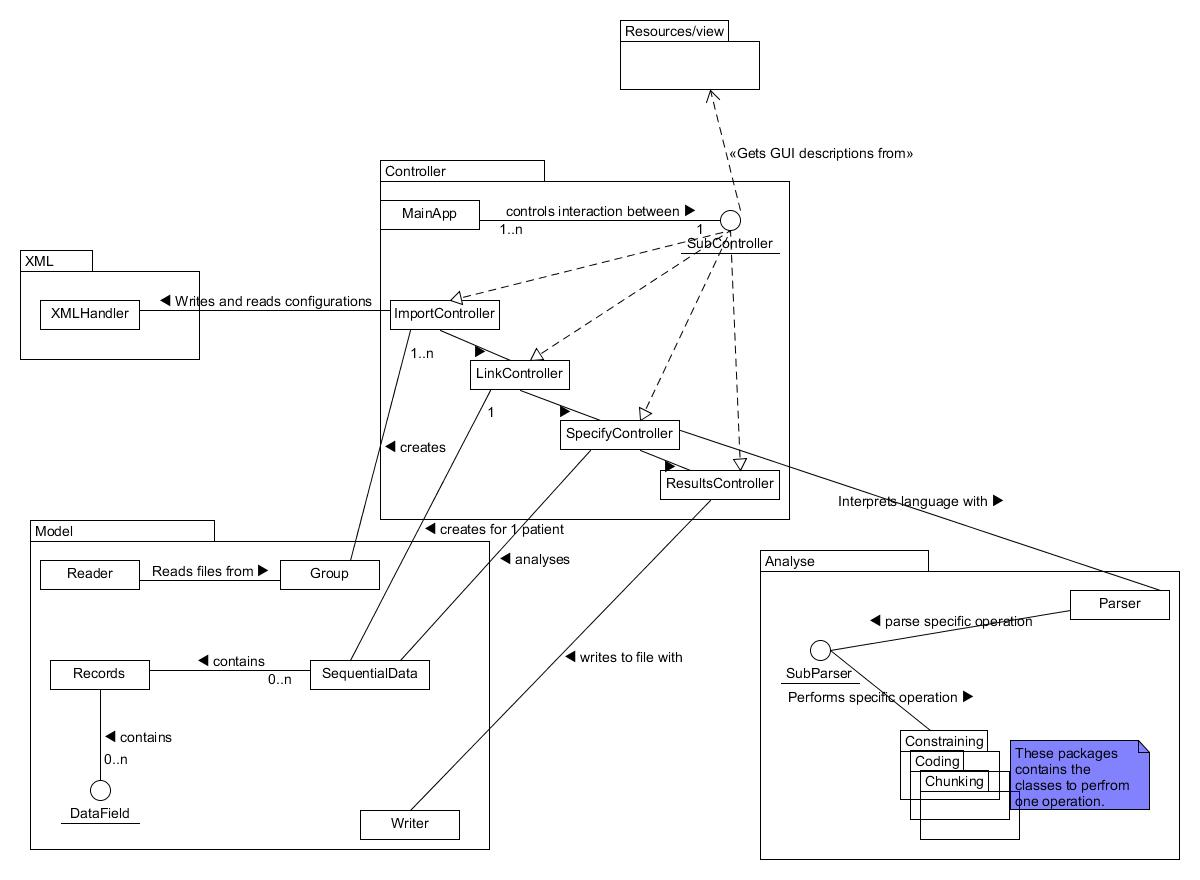
\includegraphics[width= \textwidth]{UMLdiagram}

\newpage



\underline{Alternatives to MVC}

Other architectural patterns that could be used in our situation are for example Presentation-abstraction-control, Model View Presenter, and Model View ViewModel. These patterns are interaction-oriented and similar to MVC. 

An important difference with Presentation-abstraction-control (PAC) is the abstraction component. PAC retrieves and processes the data with the Abstraction component and makes a visual presentation of the data (a template actually) with the Presentation component. The Presentation and Abstraction components never speak to each other. This communication and control flow between these components are all handled by the Control component. This is also the reason why the PAC doesn't suit our system. PAC is only useful when you aren't calling your data store directly from your display layer, which is actually what we want to do in our system. The user needs to be able to import files in the user interface. 

Model View Presenter (MVP) and Model View ViewModel (MVVM) are derivations of the MVC pattern. In MVP the controller has been replaced by a Presentation component to which all presentation logic is pushed. In MVVM this is pushed to the ViewModel. These components are responsible for exposing methods and handling all UI events by receiving input from users via the View, then process the user's data with the help of Model and passing the results back to the View. Unlike View and Controller, View and Presenter or ViewModel are completely decoupled from each other and their communication is handled through the interface. These patterns have a clean separation of the View and Model and the amount of data is reduced because of the passive View but this means that there is less encapsulation and more work to do as the developer has to do all the data binding himself. We preferred MVC above these patterns because we wanted our View to process the input partially before passing it to the next layer. This is needed for the script editor.

\underline{FXML} \\ We use FXML to provide the structure for the user interface separate from the application logic of our code. This enables us to build an interface that uses Java components without the need to worry about fetching and filling in the data. In comparison with alternatives to FXML, the scene graph in FXML is more transparent. This enables us to build and maintain a testable interface. It is also a compiled language so you do not need to recompile the code every time you want to see the changes. The content of the files will be localized as they are read so they will be automatically updated. This means that you don't have to manually update every element of your interface. Also, it's suitable for our project since FXML works with any Java Virtual Machine.  

\underline{XML Configuration} \\
We use XML to markup our data. The group configuration of files that need to be imported can be specified in an XML file. After the XML file is loaded in the program, the file groups will be filled in for the user and added visually to the program. We made a default XML configuration and added this to the program. In our program XML is also used to describe and store the data output. When stored this way, the data will not actually carry its display but its description through custom tags. The display will be extracted from the data, incorporated into a style sheet. This also means that the changes to the display of the output will not require changes to the structure of the data itself.

A few other benefits to consider are the achieved simplicity and efficiency of searching the data. Your program could parse the XML tags rather than looping through the whole file. Also, complex relationships like trees and inheritance can be easily communicated through XML. It will make the dataset more legible to a (possible) new developer with no prior knowlegde. 

Alternatives such as YAML, SGML and INI are actually easier to parse than XML, but XML is much simpler and interoperable to use. The most important advantage of XML is the "universality" of its syntax. It's easy to understand and thereby used in many applications. There are many free XML parsing libraries available in many languages. That is why probably many of our users will know how to write XML syntax, so there will be less confusion about it. 
In contrast to the alternative JSON, XML is extensible with new tags or attributes to represent the data. Since JSON is not actually a document markup language, it's not extensible. \\

\newpage 

\underline{D3.js Framework for Visualization} \\
We implemented the library D3.js in the GUI in a way it’s easy to create new graphs and add new types of graphs. It is a JavaScript library for manipulating documents based on data. It lets you build the data visualization framework that you want so it's wide in use. D3.js focuses on binding data to DOM elements and thereby makes the framework easy to use. 

An important advantage to D3.js is that it is written in JavaScript and uses a functional style which means you can reuse code and add specific functions. This means that it offers a lot of flexibility to the developer and that is exactly what we need to make the visualizations specific for this context.

An alternative to D3.js is Google Charts. It contains a lot of ready-to-use examples for all the charts and easy-to-implement features like embedding and exporting charts as pngs but it is more restricted than D3.js. With D3.js you can make your graphs the way you want. In Google Charts you can only create some of the most often used charts like frequency bars and line charts. It is also more limited in the amount of data it can handle. Google Charts will become more slow when you're working with gigabytes of data, while D3.js will stay strong. 

Even with the general graphs, you can add many other DOM functions in d3.js like zoom, click function for any graph you want which is not quite possible for all the Google Charts.



\end{itemize}






\newpage
\section{Glossary}
\textbf{Layered structure} - Also called a Multilayered Architecture; a software architecture that uses layers for allocating the different responsibilities of the program. \\ \\
\textbf{Master branch} - The version of our software application that is always ready for deployment. 



\end{document}
%%%%%%%%%%%%%%%%%%%%%%%%%%%%%%%%%%%%%%%%%%%%%%%%%%%%%%%%%%%%%%%%%%%%%%%%%%%%%%%%